\documentclass[10pt,a4paper,twocolumn,twoside]{article}
\usepackage[utf8]{inputenc}
\usepackage[catalan]{babel}
\usepackage{multicol}
\usepackage{graphicx}
\usepackage{fancyhdr}
\usepackage{times}
\usepackage{amsmath}
\usepackage{titlesec}
\usepackage{hyperref}
\usepackage{multirow}
\usepackage{float}
\usepackage{subcaption}
\usepackage{wrapfig}
\usepackage[top=2.5cm, bottom=1.3cm, left=1.2cm, right=1.2cm]{geometry}
\usepackage[figurename=Fig.,tablename=Taula,font={small,sf}]{caption}
%\usepackage[font={small,sf}]{caption}
\hypersetup{
	pdfborder={0 0 0} 
}
\usepackage{enumitem}
\setlist[itemize]{noitemsep}
\setlist[enumerate]{noitemsep}

\let\OLDthebibliography\thebibliography
\renewcommand\thebibliography[1]{
  \OLDthebibliography{#1}
  \setlength{\parskip}{0pt}
  \setlength{\itemsep}{0pt plus 0.3ex}
}

\pagestyle{fancy}
\fancyhf{}
\fancyhead[LO]{\textsf{\small $\mu$Projecte VC(GEI)-PSIV(GED), Escola d’Enginyeria (EE), Universitat Autònoma de Barcelona (UAB)}}
\fancyhead[RE]{\textsf{\small $\mu$Projecte VC(GEI)-PSIV(GED), Escola d’Enginyeria (EE), Universitat Autònoma de Barcelona (UAB)}}
\renewcommand{\headrulewidth}{0pt}

\titleformat*{\section}{\large\sffamily\scshape\bfseries}
\titleformat*{\subsection}{\normalsize\sffamily\bfseries}
\titleformat*{\subsubsection}{\normalsize\sffamily\slshape}

\begin{document}

{\sffamily
% Titol
\noindent\textbf{\LARGE ZebrAI Crossing: Detecció de passos de zebra i semàfors de vianants}
% autors
\begin{center}
Albert Capdevila Estadella (1587933), Levon Kesoyan Galstyan (1668018), Luis Martínez Zamora (1668180)
\end{center}

%\bigskip
%\bigskip
%
%\noindent 
%\textbf{Abstract} --- Lorem ipsum dolor sit amet, consectetur adipiscing elit. In auctor est et lacus luctus eleifend. Duis at tincidunt nibh. Nam sed elementum lorem, eu pretium magna. Vestibulum justo urna, imperdiet eget tristique ut, pellentesque vel turp-is. Vivamus et risus tempor, fringilla libero in, semper arcu. Praesent blandit libero vitae rutrum tincidunt. Fusce id justo quis mauris accumsan pellentesque et in massa. Nulla ut eleifend ante. Nunc pretium justo a nibh tincidunt tempus. Fusce auctor tortor nec turpis commodo, vitae posuere nulla mollis. Maecenas non placerat metus. Mauris dolor libero, laoreet quis leo vitae, dignissim lobortis enim. Curabitur in magna nibh. Aenean vel dui eros. Morbi maximus in turpis vitae fermentum.
%
%Duis interdum nisi id sem dictum rhoncus. Duis vitae ante tincidunt, tempor diam quis, tincidunt lorem. Etiam sit amet nisi tempus sapien auctor vestibulum ac eu purus. Curabi-tur a suscipit urna, sit amet facilisis erat. Morbi iaculis ves-tibulum tortor, quis varius justo mollis ut. Pellentesque plac-erat felis pretium, maximus ex quis, rutrum nisi. Sed quis imperdiet nunc. Donec euismod ipsum sed urna semper posuere. Nunc id gravida enim. Suspendisse tortor lectus, tempus tincidunt tellus at, mattis tincidunt tortor. Morbi fini-bus ultrices bibendum. Morbi ac ipsum eu erat consectetur convallis at. 
%
%\bigskip
%
%\noindent 
%\textbf{Keywords}---Image classification, noisy web data, CNNs, ubiquitous reweighting.
}
%\bigskip

%{\vrule depth 0pt height 0.5pt width 3cm\hspace{7.5pt}%
%\raisebox{-3.5pt}{\fontfamily{pzd}\fontencoding{U}\fontseries{m}\fontshape{n}\fontsize{11}{12}\selectfont\char70}%
%\hspace{7.5pt}\vrule depth 0pt height 0.5pt width 3cm\relax}
%
%\bigskip


\section{Introducció}


\textbf{ZebrAI Crossing} és un model de visió per computador que, donada una imatge en un entorn urbà, detecta si hi apareix un pas de zebra i en determina la seva orientació i posició respecte la càmera. A més a més, també detecta la presència de semàfors per a vianants i indica el seu estat (en vermell, en verd...).

\textit{Aquest és un model pensat per al desenvolupament d'OrionWay, un robot autònom que guia persones amb discapacitat visual per entorns urbans. OrionWay és un projecte de l'assignatura Robòtica, Llenguatge i Planificació del Grau en Enginyeria Informàtica a la Universitat Autònoma de Barcelona.}

\subsection{Objectius}
Donada una imatge, volem:
\vspace{-0.3em}
\begin{itemize}
	\item Identificar si hi apareix un pas de zebra.
	
	\vspace{0.3em}
	\textit{En cas afirmatiu:}
	\begin{itemize}[label=\textbullet]
		\item {Determinar l’orientació del pas de zebra.}
		\item {Determinar la posició de l'inici del pas de zebra.}
	\end{itemize}
	\item {Identificar si hi apareix un semàfor de vianants.}
	
	\vspace{0.3em}
	\textit{En cas afirmatiu:}
	\begin{itemize}[label=\textbullet]
		\item {Indicar si el semàfor es troba en verd.}
	\end{itemize}
\end{itemize}
Així doncs, aquests objectius seran útils per a posicionar i orientar el robot OrionWay quan apareguin passos de zebra, i només creuar-los quan el semàfor estigui en verd.

\section{Estat de l'art}

En el punt de partida d'aquest projecte, hem pogut trobar diversos repositoris útils i articles existents que tracten de resoldre un problema similar. Aquests són els recursos que hem investigat que ens han resultat més útils:

\subsection{Projectes}\label{sec:projectes}
\subsection*{ImVisible \cite{ImVisible}}
El projecte tracta del desenvolupament d'una aplicació mòbil que mitjançant la càmera del dispositiu analitza l'entorn per tal de detectar passos de zebra, la seva orientació i, en cas que estiguin regulats per un semàfor, detectar-ho i saber si es troba en verd o en vermell. Tot el procés de reconeixement d'imatges es fa mitjançant xarxes neuronals convolucionals.

\subsection*{Crosswalks-detection-using-YOLO \cite{CrosswalksYOLO}}
El projecte tracta del desenvolupament d'un detector de passos de zebra utilitzant YOLO, ens serà útil la resolució de problemes que s'explica al projecte, tant la unificació de les diferents deteccions que pot fer el programa a un mateix pas de zebra com la part de tenir diversitat d'exemples d'altres marques de circulació que es troben a la carretera.

\subsection*{Real-time detection of people and bicycles in pedestrian crossings - CVC \cite{CVCPedestrian}}
El projecte tracta d'una detecció instantània mitjançant una única càmera de vianants i ciclistes a passos de zebra, amb l'objectiu de poder avisar als conductors que s'apropen a l'àrea d'encreuament i altres com la necessitat de control policial, una mala configuració de semàfors...

\subsection*{PedestrianTrafficLightsAndCrosswalkDetection \cite{PedestrianDetection}}
El projecte tracta de la creació d'una xarxa neuronal convolucional per la identificació en temps real de passos de zebra i semàfors, tenint en compte l'estat d'aquest últim.


\subsection{Articles}\label{sec:articles}
\subsection*{Zebra Crossing Detection and Time Scheduling Accuracy, Enhancement Optimization Using Artificial Intelligence \cite{ZebraAI}}

Els autors proposen un sistema de detecció de passos de zebra orientat a ajudes electròniques per a persones amb discapacitat visual. La solució divideix la imatge en finestres de tamany fix que es processen seqüencialment amb un classificador de regressió logística entrenat sobre features extretes per una CNN (anomenada LYTNet). Un segon model de regressió prediu l’orientació del pas. Amb aquesta estratègia milloren la corba precision–recall respecte a enfocaments basats només en transformades de Hough i redueixen l’RMSE de l’angle estimat. No obstant això, l’enfocament patch-based incrementa el temps d’inferència i no contempla la detecció simultània de semàfors, de manera que caldria un mòdul addicional per als objectius de ZebrAI Crossing.

\subsection*{Zebra-crossing Detection for the Partially Sighted \cite{ZebraPartiallySighted}}
Aquest article relata el procés de fer un algorisme de detecció de passos de zebra, amb l'objectiu de ser útil per a Technological Aid aimed at helping Partially Sighted (TAPS). Utilitza transformacions de Hough i detecció de variacions d'intensitat per a identificar les línies paral·leles que defineixen el pas de zebra de manera precisa. A més, per aplicar restriccions que permetin diferenciar els passos de zebra de les imatges d'escales, que visualment són similars, es proven tres mètodes: la cerca d'una homografia, el càlcul de la normal mitjançant la línia de fuga obtinguda a partir de línies equidistants, i l'ús de dos punts de fuga. En tots els casos, el pendent (slope) de les escales permet diferenciar-les dels passos de zebra.

\subsection*{ZebraRecognizer: efficient and precise localization of pedestrian crossings. \cite{ZebraRecognizer}}

ZebraRecognizer està pensat per a dispositius mòbils i combina la càmera amb l’acceleròmetre per rectificar la perspectiva abans de detectar. L’algoritme segueix quatre etapes: (i) pre-processat amb suavitzat adaptatiu, (ii) càlcul de la matriu de rectificació mitjançant sensors inercials, (iii) detecció de segments de línia amb EDLines i (iv) agrupació + validació de candidats segons solapament i consistència de color. Els autors reporten 100\% de precisió amb recall 0,78 i 12 ms per imatge en escriptori (uns 32 ms en mòbil).

Aquest article encaixa molt bé amb el nostre enfocament sense deep learning perquè, primerament, la rectificació geomètrica amb els sensors del mòbil és una manera senzilla i eficaç de corregir la perspectiva abans de buscar patrons i, a més, EDLines dona línies clares i sòlides que ens ajuden a validar bé la forma dels rectangles alterns del pas de zebra.

\subsection*{Zebra-crossing detection based on cascaded Hough transform principle and vanishing point characteristics \cite{CascadedHough}}

L'article presenta un estudi per detectar passos de zebra utilitzant un filtratge de Gauss, detecció de vores de Canny i una transformada en cascada de Hough basada en el punt de fuga, sense extreure regions d'interès. També es compara amb la transformada de Hough estàndard, demostrant que la tècnica en cascada obté millors resultats.

\subsection*{Advanced Zebra Crosswalk Detection Using Deep Learning Techniques for Smart Transportation Systems \cite{ZebraImageProcessing}}

Aquest estudi amplia el problema a un escenari de trànsit intel·ligent: utilitza SSD amb transfer-learning sobre un conjunt de dades de nou classes (pas de zebra, vianants, vehicles, etc.). Demostra altes precisions i recall en temps real i planteja la seva integració en dispositius portàtils.

Encara que el cor és deep learning, la descripció inclou avaluació en temps real amb FPS i confusion matrix. La part de xarxa no és d’interès per a nosaltres, però la metodologia experimental és un bon model de validació.

\subsection*{ZebraRecognizer: Pedestrian crossing recognition for people with visual impairment or blindness \cite{RobustPedestrian}}
L'article tracta de la creació d'una aplicació mòbil que té l'objectiu de detectar passos de zebra en temps real el qual informa a l'invident mitjançant instruccions d'àudio on s'obté la informació del voltant de la persona a partir de les característiques del mòbil com l'altura, la inclinació, zoom i resolució de la càmera, etc... A la imatge obtinguda primerament es transforma en escala de grisos i s'aplica un suavitzat per reduir soroll, on posteriorment mitjançant una homografia on "desprojecta la imatge" per tal de que es trobi en un pla i així es treballi amb qualitats reals. Posteriorment apliquen una detecció de vores, utilitzant regressió ortogonal per definir una única línia comuna.

\subsection{Datasets}\label{sec:datasets}

\subsection*{Roboflow (july\_6, capstone-for-detection, capstone-for-detection1) \cite{RoboflowJuly6, RoboflowCapstone, RoboflowAugmented}}
Els tres datasets, proporcionats pel mateix usuari, contenen un gran nombre d'imatges de passos de vianants i primers plans de llums de semàfors per a vianants. Cada imatge està classificada en tres categories possibles: \texttt{green\_pedestrian\_light}, \texttt{red\_pedestrian\_light} i \texttt{zebra}, podent pertànyer a més d'una classe simultàniament. A més, per a cada classe detectada es proporciona una regió rectangular que delimita l'element corresponent (Veure Fig.~\ref{fig:classes}).
\begin{figure}[!h]
	\centering
	\begin{subfigure}{0.4\columnwidth}
		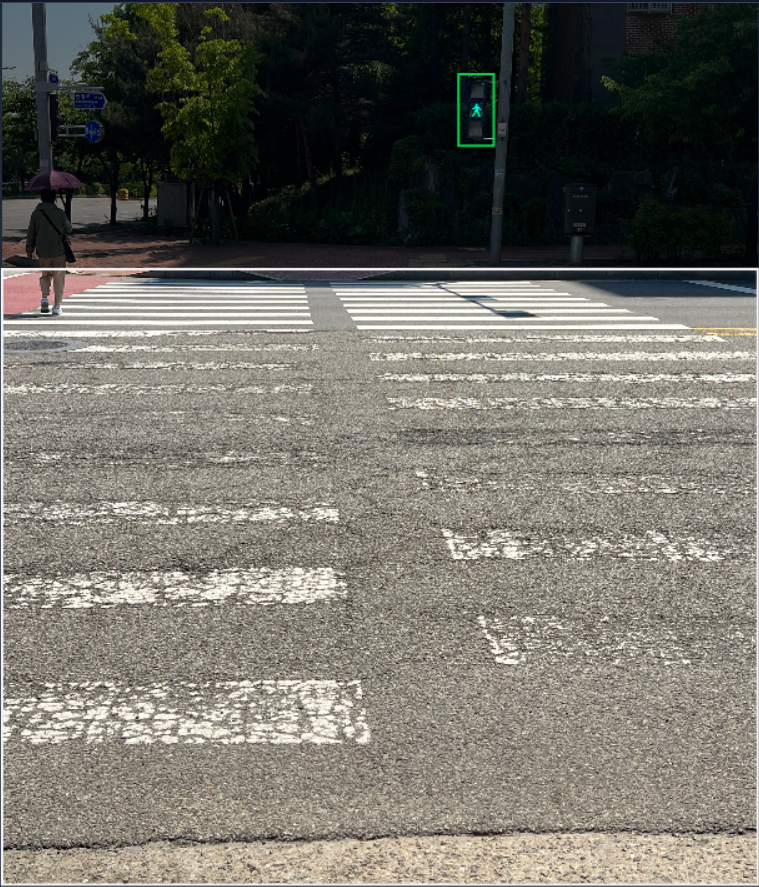
\includegraphics[width=\linewidth]{figs/1}
		\caption{Múltiples classes}
		\label{fig:classes}
	\end{subfigure}
	\quad
	\begin{subfigure}{0.46\columnwidth}
		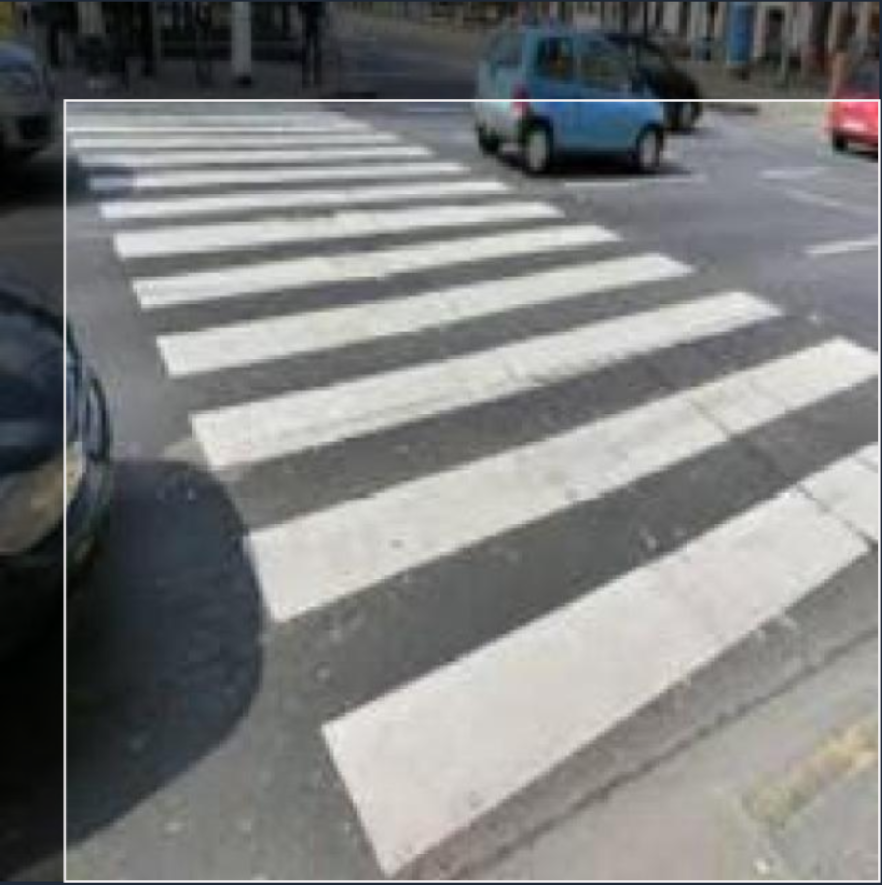
\includegraphics[width=\linewidth]{figs/2}
		\caption{Regió rectangular}
		\label{fig:regio}
	\end{subfigure}
	\caption{Exemples d'imatges dels datasets \cite{RoboflowJuly6, RoboflowCapstone, RoboflowAugmented}}
\end{figure}
\\
El gran desavantatge d'aquest conjunt de datasets és que la regió rectangular no indica l'orientació dels passos de zebra i sovint els delimita de manera recta i imprecisa (veure Fig.~\ref{fig:regio}).


\subsection*{Roboflow - crosswalk \cite{RoboflowMultiView}}
Aquest dataset és semblant als anteriors, però només inclou passos de zebra, amb regions una mica més precises. El seu principal inconvenient és que té molt poques imatges (261).


\subsection*{ImVisible \cite{ImVisible}}
El projecte ImVisible utilitza un dataset que conté imatges de passos de zebra amb semàfors per a vianants en diverses condicions, com ara dia, nit i pluja. Les imatges tenen les anotacions: \texttt{[file\_name, class, x1, y1, x2, y2, blocked tag]}, on \texttt{class} indica el tipus de llum del semàfor de vianants, \texttt{x1, y1, x2, y2} indiquen l’inici i el final de la línia perpendicular al pas de zebra en el seu punt mig, i \texttt{blocked tag} indica si el semàfor per a vianants està obstruït visualment en la imatge. L'autor del projecte proporciona les imatges del dataset en tres resolucions diferents (768x576, 876x657, 4032x3024).
\begin{figure}[!h]
	\centering
	\begin{subfigure}{0.4\columnwidth}
		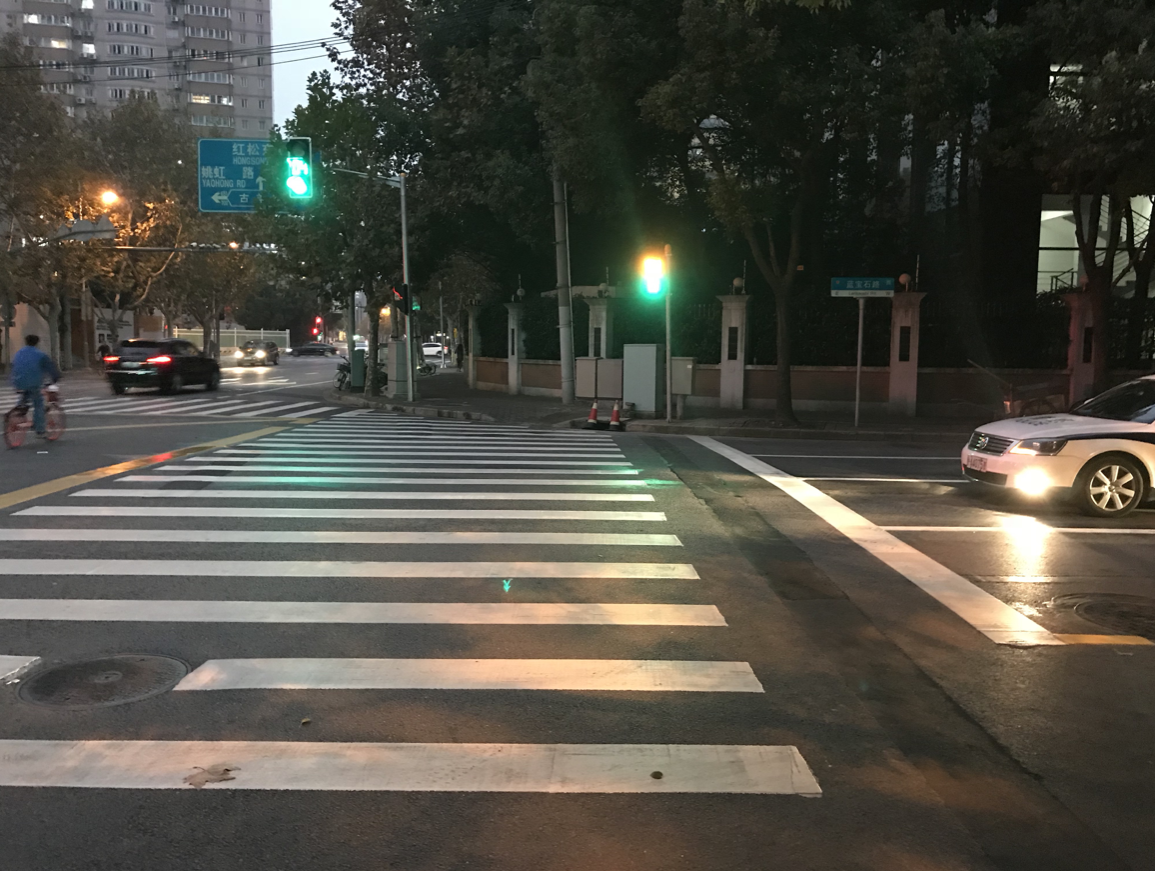
\includegraphics[width=\linewidth]{figs/3}
	\end{subfigure}
	\quad
	\begin{subfigure}{0.4\columnwidth}
		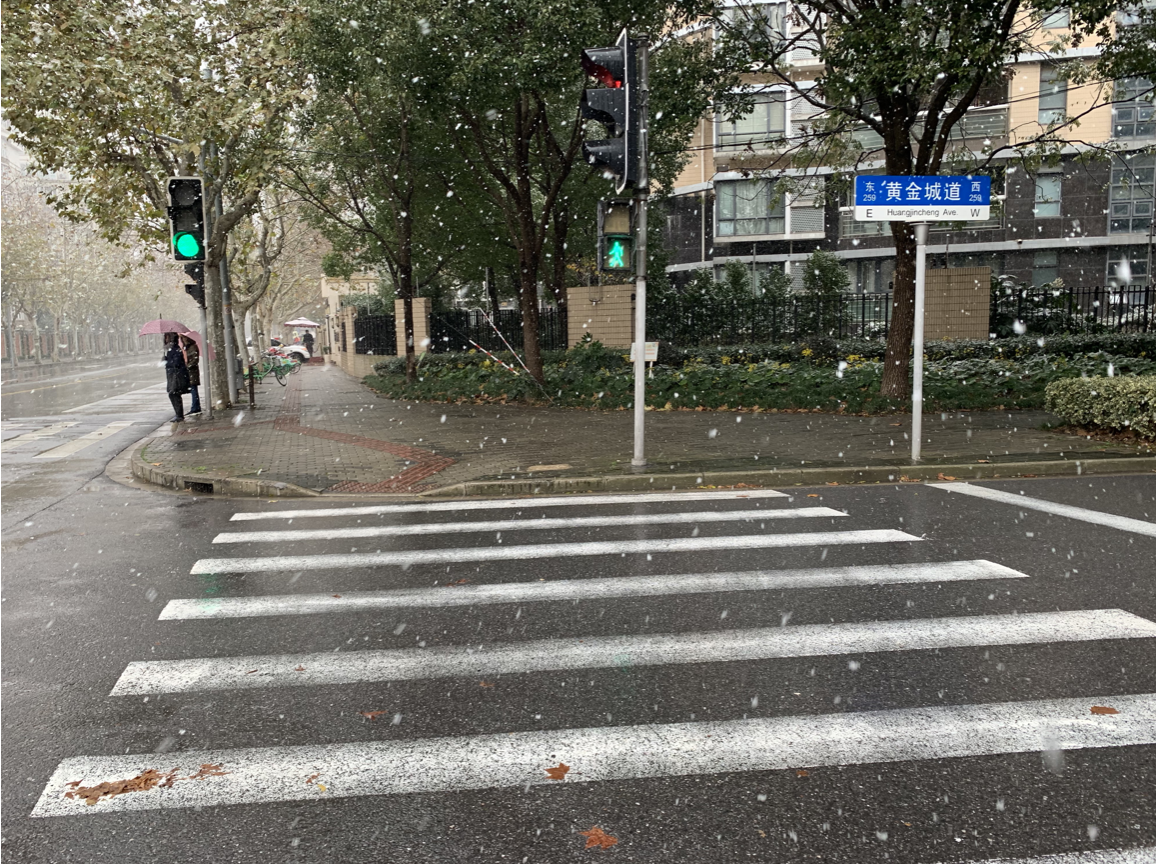
\includegraphics[width=\linewidth]{figs/4}
	\end{subfigure}
	\caption{Exemples d'imatges de ImVisible}
\end{figure}

\section{Proposta}

\subsection{Descripció de les dades}
En aquest projecte, utilitzarem un conjunt de dades fabricat a partir de dos datasets diferents trobats en repositoris de GitHub: \textbf{ImVisible \cite{ImVisible}} i \textbf{GlobalStreetscapes \cite{GlobalStreetscapes}}.
\vspace*{0.3em}
\\
Aquest conjunt de dades té dos propòsits:
\vspace*{-0.3em}
\begin{enumerate}
	\item Avaluar el rendiment de la part del model encarregada d'identificar els passos de zebra i els seus atributs.
	\item Entrenar, validar i provar la part del model encarregada d'identificar l'estat dels semàfors per a vianants.
\end{enumerate}
Hem triat el dataset d'ImVisible perquè proporciona una gran quantitat d'imatges anotades amb informació que ens permet extreure la orientació del pas de zebra, la posició de l'inici d'aquest i l'estat del semàfor de vianants.

Ara bé, per a fer una bona avaluació, també necessitarem imatges que no continguin passos de zebra, motiu pel qual hem decidit utilitzar també imatges de GlobalStreetscapes. Dins d'aquest immens conjunt de dades, hem seleccionat imatges amb els atributs \texttt{platform} = \texttt{"walking surface"}, \texttt{panoramic status} = \texttt{false}, i \texttt{view direction} = \texttt{"front"}
 per assegurar-nos que siguin similars a les de l'altre dataset.

Així doncs, hem incorporat un nou atribut als existents en el dataset d'ImVisible (Explicació a l'apartat \ref{sec:datasets}). Aquest mesura l’orientació del pas de zebra en relació amb una trajectòria recta de creuament, i es calcula a partir de la recta definida per les coordenades \texttt{(x1, y1) i (x2, y2)}:
\begin{equation*}
	\theta=atan(\frac{x_2-x_1}{y_2-y_1})
\end{equation*} 
En la aquesta figura es pot veure un exemple:
\begin{figure}[!h]
	\centering
	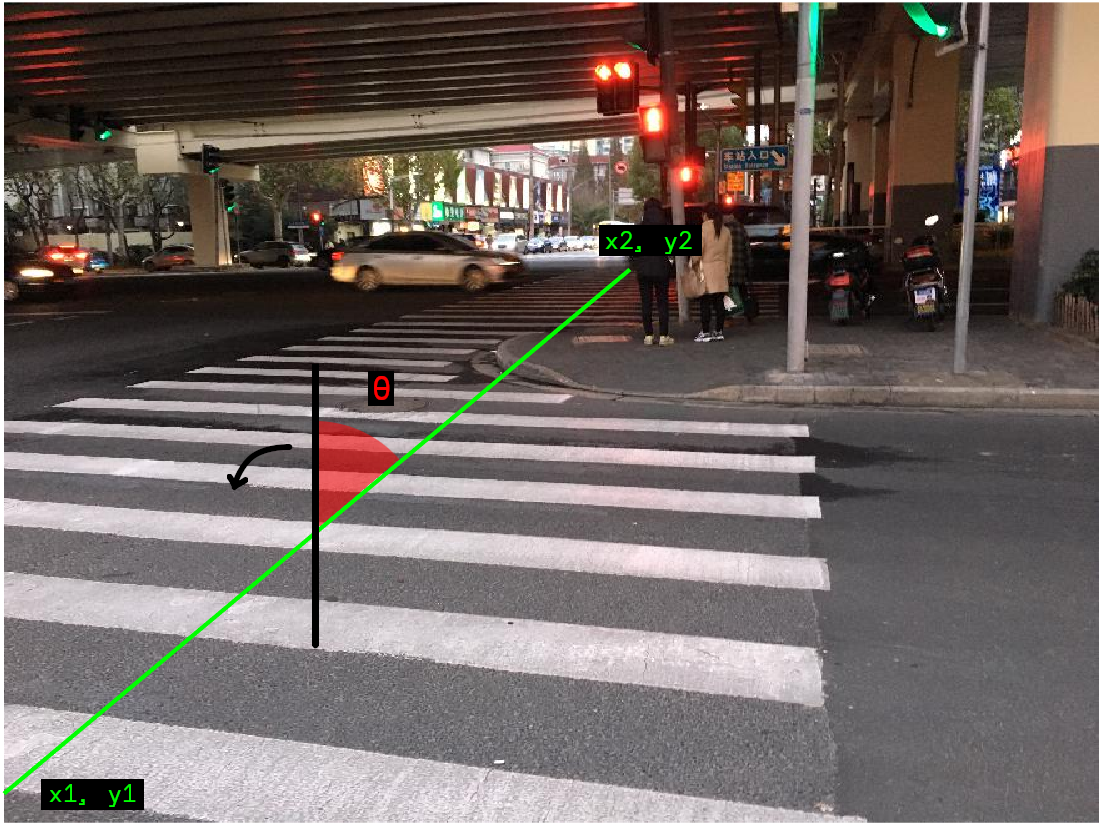
\includegraphics[width=0.95\linewidth]{figs/angle}
	\caption{Angle d'orientació del pas de zebra}
	\label{fig:angle}
\end{figure}
\\
En aquest cas, farà falta girar la càmera -$\theta$ per poder creuar el pas de zebra avançant cap endavant.\footnote{És una simplificació que no té en compte la distorsió provocada pels punts de fuga.}

A més, considerarem les coordenades (\texttt{(x1, y1) o (x2, y2)}) més properes a la càmera com el punt d'inici del pas de zebra:
\begin{equation*}
	(x, y)=(x_i, y_i : y_i > y_{3-i})
\end{equation*} 
En l'exemple anterior, \texttt{x=x1} i \texttt{y=y1}.

En conclusió, els atributs finals que té cada imatge del dataset que hem construït són: \texttt{[file\_name, x, y, theta\_rad, theta\_deg, class, blocked tag]}. \textbf{Recordatori:} \texttt{class} indica el tipus de llum del semàfor de vianants i \texttt{blocked tag} indica si el semàfor per a vianants està obstruït visualment en la imatge.

\subsection{Tècniques a utilitzar}
 
 Hem pensat que aquest projecte combinarà dues metodologies: \textbf{tècniques tradicionals} per a detectar els passos de zebra i els seus atributs, i \textbf{tècniques basades} en Deep Learning per a la detecció dels semàfors i el seu estat.
 
 Així doncs, per a la tasca de detecció dels passos de zebra, algunes de les tècniques considerades són:
 \vspace{-0.3em}
 \begin{itemize}
 	\item Detecció de vores (Laplacià, Canny,...)
 	\item Filtratge Gaussià
 	\item Morfologia matemàtica
	\item Transformades de Hough / CHT
	\item Homografies per detectar \textit{slope}
	\item Detecció de variacions de color / intensitat
 \end{itemize}
 
 En canvi, per a la detecció dels semàfors i el seu estat crearem una \textbf{xarxa neuronal (convolucional)} o bé investigarem alguna eina existent com ara \textbf{YOLO}. La idea és que utilitzarem el dataset fabricat per validar i decidir el millor model.
 
%\section{Experiments, resultats i anàlisi}


%\begin{table}[!h]
%\centering
%\begin{tabular}{lccccc}
% x & sin(x) &	cos(x)& tan(x) &  sec(x) & cosec(x)\\
%\hline
%30$^\circ$ & 0.5000 & 0.8660 & 0.5774 & 1.1547 & 2.0000\\
%45$^\circ$ & 0.7071 & 0.7071 & 1.0000 & 1.4142 & 1.4142\\
%60$^\circ$ & 0.8660 & 0.5000 & 1.7321 & 2.0000 & 1.1547\\
%\hline
%\end{tabular}
%\caption{ Raons trigonomètriques per diferents valors d’angles.}
%\label{t:raonstrigonometriques}
%\end{table}


%\section{Conclusions}


\begin{thebibliography}{9}
	
	\subsection*{Projectes}
	\bibitem{ImVisible}
	S. Yu et al., \textit{\href{https://github.com/samuelyu2002/ImVisible}{ImVisible: Pedestrian Traffic Light Dataset, LytNet Neural Network, and Mobile Application for the Visually Impaired}}. GitHub repository.
	
	\bibitem{CrosswalksYOLO}
	N. Kuznetsov, \textit{\href{https://github.com/xN1ckuz/Crosswalks-Detection-using-YOLO}{Crosswalks Detection using YOLO: A Supervised Method for Detecting Pedestrian Crosswalks}}. GitHub repository.
	
	\bibitem{CVCPedestrian}
	CVC UAB, \textit{\href{https://www.cvc.uab.es/portfolio/?page_id=3872}{Real-time detection of people and bicycles in pedestrian crossings}}.
	
	\bibitem{PedestrianDetection}
	R. Santos, \textit{\href{https://github.com/ronaldosm/PedestrianTrafficLightsAndCrosswalkDetection}{PedestrianTrafficLightsAndCrosswalkDetection}}. GitHub repository.
	
	\subsection*{Articles}
	\bibitem{ZebraAI}
	M. A. Rahman et al., \textit{\href{https://www.researchgate.net/publication/354299232_Zebra_Crossing_Detection_and_Time_Scheduling_Accuracy_Enhancement_Optimization_Using_Artificial_Intelligence}{Zebra Crossing Detection and Time Scheduling Accuracy Enhancement Optimization Using Artificial Intelligence}}. ResearchGate, 2021.
	
	\bibitem{ZebraPartiallySighted}
	D. Bradley and A. Dunlop, \textit{\href{https://scispace.com/pdf/zebra-crossing-detection-for-the-partially-sighted-22q9n427id.pdf}{Zebra Crossing Detection for the Partially Sighted}}.
	
	\bibitem{ZebraRecognizer}
	D. Ahmetovic et al., \textit{\href{https://dragan.ahmetovic.it/pdf/ahmetovic2014zebrarecognizer.pdf}{ZebraRecognizer: efficient and precise localization of pedestrian crossings.}}. 2014.
	
	\bibitem{CascadedHough}
	J. Zhang and L. Wang, \textit{\href{https://www.degruyterbrill.com/document/doi/10.1515/comp-2022-0260/html}{Zebra-crossing detection based on cascaded Hough transform principle and vanishing point characteristics}}. De Gruyter, 2022.
	
	\bibitem{ZebraImageProcessing}
	P. Sharma and R. K. Singh, \textit{\href{https://www.ijese.org/wp-content/uploads/Papers/v13i3/B104214020125.pdf}{Zebra Crossing Detection using Image Processing Techniques}}. IJESE, 2022.
	
	\bibitem{RobustPedestrian}
	Y. Chen et al., \textit{\href{https://www.sciencedirect.com/science/article/abs/pii/S0031320316300826}{ZebraRecognizer: Pedestrian crossing recognition for people with visual impairment or blindness}}. Pattern Recognition, 2016.
	
	\subsection*{Datasets}
	
	\bibitem{RoboflowJuly6}
	Dkdkd. \href{https://universe.roboflow.com/dkdkd/july_6}{\textit{july\_6 Dataset}}. Roboflow Universe, juny 2024.
	
	\bibitem{RoboflowCapstone}
	Dkdkd. \href{https://universe.roboflow.com/dkdkd/capstone-for-detection}{\textit{capstone for detection Dataset}}. Roboflow Universe, juny 2024.
	
	\bibitem{RoboflowAugmented}
	Dkdkd. \href{https://universe.roboflow.com/dkdkd/capstone-for-detection1}{\textit{capstone for detection1 Dataset}}. Roboflow Universe, juny 2024.
	
	\bibitem{RoboflowMultiView}
	Esera. \href{https://universe.roboflow.com/esera/crosswalk-cz3sx}{\textit{crosswalk Dataset}}. Roboflow Universe, agost 2024.
	
	\bibitem{GlobalStreetscapes}
	UALSG. \href{https://github.com/ualsg/global-streetscapes}{\textit{Global Streetscapes Dataset for Crosswalk Detection}}. GitHub repository.
	
	
	
\end{thebibliography}
\end{document}

